\documentclass[journal]{IEEEtran}
% \documentclass[journal,12pt,onecolumn,draftclsnofoot]{IEEEtran}

\usepackage[table]{xcolor}
\usepackage{adjustbox}
\usepackage{algorithm}
\usepackage{algpseudocode}
\usepackage{amsfonts}
\usepackage{amsmath}
\usepackage{amssymb}
\usepackage{amsthm}
\usepackage{bookmark}
\usepackage{booktabs}
\usepackage[makeroom]{cancel}
\usepackage[american]{circuitikz}
\usepackage{cite}
\usepackage{fixmath}
\usepackage[acronym]{glossaries-extra}
\usepackage{hyperref}
\usepackage{import}
\usepackage{mathtools}
\usepackage{microtype}
\usepackage[short]{optidef}
\usepackage{pgfplots}
\usepackage{ragged2e}
\usepackage[subtle]{savetrees}
\usepackage{siunitx}
\usepackage{stfloats}
\usepackage[caption=false,font=footnotesize,subrefformat=parens,labelformat=parens]{subfig}
\usepackage{tabularx}
\usepackage{tikz}
\usepackage{graphicx}
\usepackage{epstopdf}

% page limit hacks
% \usepackage{setspace}
% ! \usepackage[top=1cm, bottom=1cm, left=1cm, right=1cm]{geometry}
% \abovedisplayskip=1mm
% \belowdisplayskip=1mm
% \abovedisplayshortskip=1mm
% \belowdisplayshortskip=1mm
% \setlength{\jot}{0.1mm}
% \setlength{\floatsep}{1mm}
% \setlength{\textfloatsep}{1mm}
% \setlength{\intextsep}{1mm}
% \setlength{\skip\footins}{2mm}


% amsthm
\newtheorem{proposition}{Proposition}
\newtheorem{remark}{Remark}

% PGF/TikZ
\usetikzlibrary{arrows,calc,matrix,patterns,plotmarks,positioning,shapes}
\usetikzlibrary{decorations.pathmorphing,decorations.pathreplacing,decorations.shapes,shapes.geometric}
\usepgfplotslibrary{groupplots,patchplots}
\pgfplotsset{compat=newest}

% tabularx, ragged2e
\newcolumntype{L}{>{\RaggedRight}X}
\newcolumntype{C}{>{\centering\arraybackslash}X}
\renewcommand\tabularxcolumn[1]{m{#1}}

% algpseudocode
\makeatletter
\renewcommand{\fnum@algorithm}{\fname@algorithm{} \thealgorithm:}
\newcommand\setalgorithmcaptionfont[1]{%
	\let\my@floatc@ruled\floatc@ruled          % save \floatc@ruled
	\def\floatc@ruled{%
		\global\let\floatc@ruled\my@floatc@ruled % restore \floatc@ruled
		#1\floatc@ruled}}
\makeatother

\algrenewcommand{\algorithmicrequire}{\textbf{Input:}}
\algrenewcommand{\algorithmicensure}{\textbf{Output:}}
\algrenewcommand{\algorithmicwhile}{\textbf{While}}
\algrenewcommand{\algorithmicend}{\textbf{End}}
\algrenewcommand{\algorithmicrepeat}{\textbf{Repeat}}
\algrenewcommand{\algorithmicuntil}{\textbf{Until}}
\algrenewcommand{\algorithmicfor}{\textbf{For}}
\algrenewcommand{\algorithmicdo}{}

% glossaries-extra
\glsdisablehyper
\setabbreviationstyle[acronym]{long-short}
\newacronym{ao}{AO}{Alternating Optimization}
\newacronym{bd}{BD}{Beyond-Diagonal}
\newacronym{dof}{DoF}{Degree of Freedom}
\newacronym{mimo}{MIMO}{Multiple-Input Multiple-Output}
\newacronym{rcg}{RCG}{Riemannian Conjugate Gradient}
\newacronym{ris}{RIS}{Reconfigurable Intelligent Surface}
\newacronym{pc}{PC}{Point-to-point Channel}
\newacronym{ic}{IC}{Interference Channel}
\newacronym{snr}{SNR}{Signal-to-Noise Ratio}

\begin{document}
\title{Channel Shaping Using Reconfigurable Intelligent Surfaces: From Diagonal to Beyond}
\author{
	\IEEEauthorblockN{
		Yang~Zhao,~\IEEEmembership{Member,~IEEE,}
		Hongyu~Li,~\IEEEmembership{Graduate Student Member,~IEEE,}\\
		Yijie~Mao,~\IEEEmembership{Member,~IEEE,}
		Shanpu~Shen,~\IEEEmembership{Member,~IEEE,}
		and~Bruno~Clerckx,~\IEEEmembership{Fellow,~IEEE}
	}
	% \thanks{
	% 	The authors are with the Department of Electrical and Electronic Engineering, Imperial College London, London SW7 2AZ, U.K. (e-mail: \{yang.zhao18, b.clerckx\}@imperial.ac.uk).
	% 	B. Clerckx is also with Silicon Austria Labs (SAL), Graz A-8010, Austria.
	% }
}
\maketitle

% \begin{abstract}
% \end{abstract}

% \begin{IEEEkeywords}
% \end{IEEEkeywords}

\glsresetall

\begin{section}{Assumption}
	We introduce \gls{bd} \gls{ris} in \gls{mimo} \gls{pc} and \gls{ic}.
	% point-to-point and interference \gls{mimo} channels.
	All proposals are based on assumption of \emph{asymmetric} passive \gls{bd} \gls{ris}, i.e., symmetry constraint $\mathbf{\Theta}_g = \mathbf{\Theta}_g^\mathsf{T}$ is relaxed.
	This is feasible when asymmetric passive components (e.g., ring hybrids and branch-line hybrids) \cite{Ahn2006} are available.
	This assumption was also made in Hongyu's papers \cite{Li2023b,Li2023c}.
	For quadratic problems, the proposed algorithms may be extended to symmetric \gls{bd} \gls{ris} by replacing singular value decomposition with Takagi factorization \cite{Horn2012}.
\end{section}

\begin{section}{\glsentryshort{mimo}-\glsentryshort{pc}}
	\begin{subsection}{Channel Power Maximization}
		Consider a \gls{bd} \gls{ris} with $N^\mathrm{S}$ elements, which is divided into $G$ groups of equal $L$ elements.
		\begin{maxi!}
			{\scriptstyle{\mathbf{\Theta}}}{\left\lVert \mathbf{H}^\mathrm{D} + \sum_g\nolimits \mathbf{H}_g^\mathrm{B} \mathbf{\Theta}_g \mathbf{H}_g^\mathrm{F} \right\rVert _\mathrm{F}^2}{\label{op:pc_power}}{}
			\addConstraint{\mathbf{\Theta}_g^\mathsf{H} \mathbf{\Theta}_g=\mathbf{I}, \quad \forall g \in \mathcal{G} \triangleq \{1,\ldots,G\}.}{}{}
		\end{maxi!}
		For \emph{symmetric} BD-RIS, the problem has been solved in
		\begin{itemize}
			\item Matteo's paper \cite{Nerini2023}: SISO and equivalent\footnote{Single-stream MIMO with given precoder and combiner.};
			\item Ignacio's paper \cite{Santamaria2023}: SISO and directless MISO/SIMO.
		\end{itemize}

		\begin{remark}
			% The difficulty of \eqref{op:pc_power} is that the \gls{ris} needs to balance the (additive) direct-indirect eigenspace alignment and the (multiplicative) forward-backward eigenspace alignment.
			The difficulty of \eqref{op:pc_power} is that the \gls{ris} needs to balance the additive (direct-indirect) and multiplicative (forward-backward) eigenspace alignment.
			% align the direct and indirect eigenspaces while preserving the
			Interestingly, it has the same form as the \emph{weighted orthogonal Procrustes problem} \cite{Gower2004}:
			\begin{mini!}
				{\scriptstyle{\mathbf{\Theta}}}{\lVert \mathbf{C} - \mathbf{A \Theta B} \rVert _\mathrm{F}^2}{\label{op:weighted_orthogonal_procrustes}}{}
				\addConstraint{\mathbf{\Theta}^\mathsf{H} \mathbf{\Theta}=\mathbf{I}.}{}{}
			\end{mini!}
			There exists no trivial solution to \eqref{op:weighted_orthogonal_procrustes}.
			One lossy transformation, by moving $\mathbf{\Theta}$ to one side \cite{Bell2003}, formulates a standard orthogonal Procrustes problem:
			\begin{mini!}
				{\scriptstyle{\mathbf{\Theta}}}{\lVert \mathbf{A}^\dagger \mathbf{C} - \mathbf{\Theta B} \rVert _\mathrm{F}^2}{\label{op:standard_orthogonal_procrustes}}{}
				\addConstraint{\mathbf{\Theta}^\mathsf{H} \mathbf{\Theta}=\mathbf{I}.}{}{}
			\end{mini!}
			\eqref{op:standard_orthogonal_procrustes} has a global optimal solution $\mathbf{\Theta}^\star = \mathbf{U} \mathbf{V}^\mathsf{H}$, where $\mathbf{U}$ and $\mathbf{V}$ are left and right singular matrix of $\mathbf{\mathbf{A}^\dagger \mathbf{C} \mathbf{B}^\mathsf{H}}$ \cite{Golub2013}.
			This low-complexity solution will be compared with the one proposed later.
		\end{remark}

		Inspired by \cite{Nie2017}, we propose an iterative algorithm to solve \eqref{op:pc_power}.
		The idea is to successively approximate the quadratic objective with a sequence of affine functions and solve the resulting subproblems in closed form.

		\begin{proposition}
			Start from any $\mathbf{\Theta}^{(0)}$, the sequence
			\begin{equation}
				\mathbf{\Theta}_g^{(r+1)} = \mathbf{U}_g^{(r)} \mathbf{V}_g^{(r)}, \quad \forall g
			\end{equation}
			converges to a stationary point of \eqref{op:pc_power}, where $\mathbf{U}_g^{(r)}$ and $\mathbf{V}_g^{(r)}$ are left and right singular matrix of
			\begin{equation}
				\begin{split}
					\mathbf{M}_g^{(r)}
					& = {\mathbf{H}_g^\mathrm{B}}^\mathsf{H} \mathbf{H}^\mathrm{D} {\mathbf{H}_g^\mathrm{F}}^\mathsf{H} + \sum_{g' < g} {\mathbf{H}_{g'}^\mathrm{B}}^\mathsf{H} \mathbf{H}_{g'}^\mathrm{B} \mathbf{\Theta}_{g'}^{(r+1)} \mathbf{H}_{g'}^\mathrm{F} {\mathbf{H}_{g'}^\mathrm{F}}^\mathsf{H} \\
					& \quad + \sum_{g' \ge g} {\mathbf{H}_{g'}^\mathrm{B}}^\mathsf{H} \mathbf{H}_{g'}^\mathrm{B} \mathbf{\Theta}_{g'}^{(r)} \mathbf{H}_{g'}^\mathrm{F} {\mathbf{H}_{g'}^\mathrm{F}}^\mathsf{H}.
				\end{split}
			\end{equation}
		\end{proposition}

		\begin{proof}
			To be added.
		\end{proof}

		\begin{figure}[!t]
			\centering
			\resizebox{0.65\columnwidth}{!}{
				% This file was created by matlab2tikz.
%
%The latest updates can be retrieved from
%  http://www.mathworks.com/matlabcentral/fileexchange/22022-matlab2tikz-matlab2tikz
%where you can also make suggestions and rate matlab2tikz.
%
\definecolor{mycolor1}{rgb}{0.85098,0.32549,0.09804}%
\definecolor{mycolor2}{rgb}{0.92941,0.69412,0.12549}%
\definecolor{mycolor3}{rgb}{0.49412,0.18431,0.55686}%
\definecolor{mycolor4}{rgb}{0.46667,0.67451,0.18824}%
%
\begin{tikzpicture}

\begin{axis}[%
width=7.607cm,
height=6cm,
at={(0cm,0cm)},
scale only axis,
xmin=0,
xmax=8,
xtick={0,1,2,3,4,5,6,7,8},
xticklabels={{$2^0$},{$2^1$},{$2^2$},{$2^3$},{$2^4$},{$2^5$},{$2^6$},{$2^7$},{$2^8$}},
xlabel style={font=\color{white!15!black}},
xlabel={RIS Group Size},
ymin=0,
ymax=7e-05,
ylabel style={font=\color{white!15!black}},
ylabel={Channel Power [W]},
axis background/.style={fill=white},
xmajorgrids,
ymajorgrids,
legend style={at={(0.03,0.97)}, anchor=north west, legend cell align=left, align=left, draw=white!15!black}
]
\addplot [color=black, line width=2.0pt]
  table[row sep=crcr]{%
0	9.99481299849178e-06\\
8	9.99481299849178e-06\\
};
\addlegendentry{$N_s = 0$}

\addplot [color=mycolor1, dashed, line width=2.0pt, mark=+, mark options={solid, mycolor1}]
  table[row sep=crcr]{%
0	1.02065060534792e-05\\
1	1.02857052718835e-05\\
2	1.03657178891351e-05\\
};
\addlegendentry{$N_s = 4$}

\addplot [color=mycolor2, dotted, line width=2.0pt, mark=square, mark options={solid, mycolor2}]
  table[row sep=crcr]{%
0	1.08240394393943e-05\\
1	1.11240963559512e-05\\
2	1.14708685265676e-05\\
3	1.16901587097421e-05\\
4	1.17920396956223e-05\\
};
\addlegendentry{$N_s = 16$}

\addplot [color=mycolor3, dashdotted, line width=2.0pt, mark=x, mark options={solid, mycolor3}]
  table[row sep=crcr]{%
0	1.38635087399098e-05\\
1	1.53706530394954e-05\\
2	1.70408162342293e-05\\
3	1.82388146554718e-05\\
4	1.88521652325586e-05\\
5	1.92013834134077e-05\\
6	1.93951032304193e-05\\
};
\addlegendentry{$N_s = 64$}

\addplot [color=mycolor4, line width=2.0pt, mark=triangle, mark options={solid, mycolor4}]
  table[row sep=crcr]{%
0	2.97266633680327e-05\\
1	3.79660436735737e-05\\
2	4.94606552637649e-05\\
3	5.8335214274755e-05\\
4	6.30806269398545e-05\\
5	6.56210846273517e-05\\
6	6.68339320816644e-05\\
7	6.76530541601078e-05\\
8	6.88056961056934e-05\\
};
\addlegendentry{$N_s = 256$}

\end{axis}

\begin{axis}[%
width=9.816cm,
height=7.362cm,
at={(-1.276cm,-0.81cm)},
scale only axis,
xmin=0,
xmax=1,
ymin=0,
ymax=1,
axis line style={draw=none},
ticks=none,
axis x line*=bottom,
axis y line*=left
]
\end{axis}
\end{tikzpicture}%
			}
			\caption{Average channel power versus \gls{ris} elements $N^\mathrm{S}$ and group size $L$ for $(N^\mathrm{T}, N^\mathrm{R}) = (8, 4)$, $(\Lambda^\mathrm{D}, \Lambda^\mathrm{F}, \Lambda^\mathrm{B}) = (65, 54, 46) \unit{dB}$.}
			\label{sm:pc_power_sx}
		\end{figure}

		\begin{figure}[!t]
			\centering
			\subfloat[Without Direct Link\label{sm:pc_power_bond_nd}]{
				\resizebox{0.48\columnwidth}{!}{
					% This file was created by matlab2tikz.
%
%The latest updates can be retrieved from
%  http://www.mathworks.com/matlabcentral/fileexchange/22022-matlab2tikz-matlab2tikz
%where you can also make suggestions and rate matlab2tikz.
%
\definecolor{mycolor1}{rgb}{0.46667,0.67451,0.18824}%
\definecolor{mycolor2}{rgb}{0.92941,0.50588,0.59608}%
%
\begin{tikzpicture}

\begin{axis}[%
width=7.607cm,
height=6cm,
at={(0cm,0cm)},
scale only axis,
bar shift auto,
xmin=0,
xmax=6,
xtick={1,2,3,4,5},
xticklabels={{1},{4},{16},{64},{256}},
xlabel style={font=\color{white!15!black}},
xlabel={RIS Group Size},
ymin=0,
ymax=3.5e-05,
ylabel style={font=\color{white!15!black}},
ylabel={Channel Power [W]},
axis background/.style={fill=white},
xmajorgrids,
ymajorgrids,
legend style={at={(0.03,0.97)}, anchor=north west, legend cell align=left, align=left, draw=white!15!black}
]
\addplot[ybar, bar width=0.8, fill=mycolor1, draw=black, area legend] table[row sep=crcr] {%
1	7.67624350482862e-07\\
2	1.32530638063741e-06\\
3	3.06197930445936e-06\\
4	9.39519835024894e-06\\
5	3.02284526139409e-05\\
};
\addplot[forget plot, color=white!15!black] table[row sep=crcr] {%
0	0\\
6	0\\
};
\addlegendentry{Composite}

\addplot [color=black, line width=2.0pt]
  table[row sep=crcr]{%
-0.2	0\\
6.2	0\\
};
\addlegendentry{Direct}

\addplot [color=mycolor2, line width=2.0pt]
  table[row sep=crcr]{%
-0.2	3.04194803196479e-05\\
6.2	3.04194803196479e-05\\
};
\addlegendentry{Cascaded}

\end{axis}
\end{tikzpicture}%
				}
			}
			\subfloat[With Direct Link\label{sm:pc_power_bond_hd}]{
				\resizebox{0.48\columnwidth}{!}{
					% This file was created by matlab2tikz.
%
%The latest updates can be retrieved from
%  http://www.mathworks.com/matlabcentral/fileexchange/22022-matlab2tikz-matlab2tikz
%where you can also make suggestions and rate matlab2tikz.
%
\definecolor{mycolor1}{rgb}{0.46667,0.67451,0.18824}%
\definecolor{mycolor2}{rgb}{0.92941,0.50588,0.59608}%
%
\begin{tikzpicture}

\begin{axis}[%
width=7.607cm,
height=6cm,
at={(0cm,0cm)},
scale only axis,
bar shift auto,
xmin=0,
xmax=6,
xtick={1,2,3,4,5},
xticklabels={{1},{4},{16},{64},{256}},
xlabel style={font=\color{white!15!black}},
xlabel={RIS Group Size},
ymin=0,
ymax=7e-05,
ylabel style={font=\color{white!15!black}},
ylabel={Channel Power [W]},
axis background/.style={fill=white},
xmajorgrids,
ymajorgrids,
legend style={at={(0.03,0.97)}, anchor=north west, legend cell align=left, align=left, draw=white!15!black}
]
\addplot[ybar, bar width=0.8, fill=mycolor1, draw=black, area legend] table[row sep=crcr] {%
1	2.83336295997331e-05\\
2	4.76924466169225e-05\\
3	6.08890936283682e-05\\
4	6.46004645413477e-05\\
5	6.64188484186803e-05\\
};
\addplot[forget plot, color=white!15!black] table[row sep=crcr] {%
0	0\\
6	0\\
};
\addlegendentry{Composite}

\addplot [color=black, line width=2.0pt]
  table[row sep=crcr]{%
-0.2	9.51300474293446e-06\\
6.2	9.51300474293446e-06\\
};
\addlegendentry{Direct}

\addplot [color=mycolor2, line width=2.0pt]
  table[row sep=crcr]{%
-0.2	3.07152044114707e-05\\
6.2	3.07152044114707e-05\\
};
\addlegendentry{Cascaded}

\end{axis}
\end{tikzpicture}%
				}
			}
			\caption{Average channel power versus \gls{ris} group size $L$ for $(N^\mathrm{T}, N^\mathrm{S}, N^\mathrm{R}) = (8, 256, 4)$, $(\Lambda^\mathrm{D}, \Lambda^\mathrm{F}, \Lambda^\mathrm{B}) = (65, 54, 46) \unit{dB}$.}
			\label{sm:pc_power_bond}
		\end{figure}
		% Fig.~\ref{sm:pc_power_sx} shows that, apart from numerous reflecting elements, a sufficiently large group size can help
		% Fig.~\ref{sm:pc_power_sx} shows that increasing the group size can improve the channel power especially for a large \gls{ris}.
		Fig.~\ref{sm:pc_power_sx} shows that, apart from adding reflecting elements $N^\mathrm{S}$, increasing the group size $L$ also improves the channel power.
		% The behavior is more obvious for a large \gls{ris}.
		This behavior is more pronounced for a large \gls{ris}.
		For example, the gain of pairwise connection is \qty{2.8}{\percent} for $N^\mathrm{S} = 16$ and \qty{28}{\percent} for $N^\mathrm{S} = 256$.
		% \gls{bd} \gls{ris} provides a higher channel power than conventional \gls{ris}.
		% As $L$ increases from 1 to 2,
		It implies that the channel shaping capability of \gls{bd} \gls{ris} scales with group size $L$.

		Fig.~\ref{sm:pc_power_bond_hd} and \ref{sm:pc_power_bond_nd} compare the average channel power without and with direct link.
		% where the cascaded channel power available to passive \gls{ris} is $\lVert \mathbf{H}^\mathrm{B} \rVert _\mathrm{F}^2 \lVert \mathbf{H}^\mathrm{F} \rVert _\mathrm{F}^2$.
		% where the cascaded channel power available to passive \gls{ris} is $\lVert \mathbf{H}^\mathrm{B} \rVert _\mathrm{F}^2 \lVert \mathbf{H}^\mathrm{F} \rVert _\mathrm{F}^2$.
		% ``Cascaded'' means the maximum power of the cascaded channel, i.e., $\lVert \mathbf{H}^\mathrm{B} \rVert _\mathrm{F}^2 \lVert \mathbf{H}^\mathrm{F} \rVert _\mathrm{F}^2$.
		% maximum power of the cascaded channel, i.e., $\lVert \mathbf{H}^\mathrm{B} \rVert _\mathrm{F}^2 \lVert \mathbf{H}^\mathrm{F} \rVert _\mathrm{F}^2$.
		% ? ``Cascaded'' means the \emph{power product} of the forward and backward channels.
		% ``Cascaded'' means the sum of element-wise product of first $N = \min(N^\mathrm{T}, N^\mathrm{S}, N^\mathrm{R})$ eigenvalues of the forward and backward channels.
		``Cascaded'' means the sum of element-wise product of first $N = \min(N^\mathrm{T}, N^\mathrm{S}, N^\mathrm{R})$ eigenvalues (i.e., element-wise power product) of the forward and backward channels.
		We observe that diagonal \gls{ris} wastes substantial cascaded power and struggles to align the direct-indirect eigenspace.
		When the direct link is absent, only \qty{2.6}{\percent} of available power is utilized by diagonal \gls{ris} while \qty{100}{\percent} power is recycled by fully-connected \gls{ris}.
		When the direct link is present, the proposed \gls{bd} \gls{ris} design can balance the direct-indirect and forward-backward eigenspace alignment for an optimal channel boost.
		It is worth noting that, when $L$ is sufficiently large, the composite channel power surpasses the power sum of direct and cascaded channels, thanks to the constructive \emph{amplitude superposition} of direct and cascaded channels.
		This again emphasizes the advantage of in-group connection of \gls{bd} \gls{ris}.
		% This is because the direct and indirect channels superpose
		% the proposed \gls{bd} \gls{ris} design can also be applied to conventional \gls{ris} to improve the channel power.
		% When the direct link is present, a small $L$ cannot align the direct-indirect eigenspace.

		% neither effectively utilizes the cascaded channel power, nor effectively align the direct-indirect eigenspace.
		% We observe that conventional \gls{ris} neither effectively utilizes the cascaded channel power, nor effectively align the direct-indirect eigenspace.
		% For conventional \gls{ris},
		% align the direct-indirect eigenspace.
		% When the direct link is present, a small $L$ can neither align the direct-indirect eigenspace nor the forward-backward eigenspace.
		% For a relatively large $N^\mathrm{S}$, conventional \gls{ris} cannot
		% neither the direct-indirect nor the forward-backward eigenspace can be effectively aligned with a small $L$.

		% When the direct link is present, a small $L$ can neither preserve the
		% neither align the direct-indirect eigenspace nor the forward-backward eigenspace.

		% When the direct link is absent, a large $L$ can align the forward-backward eigenspace but cannot preserve the forward-backward power balance.
	\end{subsection}

	\begin{subsection}{Rate Maximization}
		The problem is formulated w.r.t. precoder (instead of transmit covariance matrix) for reference:
		\begin{maxi!}
			{\scriptstyle{\mathbf{W},\mathbf{\Theta}}}{\log \det \biggl(\mathbf{I} + \frac{\mathbf{W}^\mathsf{H}\mathbf{H}^\mathsf{H}\mathbf{H}\mathbf{W}}{\sigma_n^2}\biggr)}{\label{op:pc_rate}}{\label{ob:pc_rate}}
			\addConstraint{\lVert \mathbf{W} \rVert _\mathrm{F}^2 \le P}{}{}
			\addConstraint{\mathbf{\Theta}_g^\mathsf{H} \mathbf{\Theta}_g=\mathbf{I}, \quad \forall g.}{}{\label{cs:pc_rate_unitary}}
		\end{maxi!}

		\eqref{op:pc_rate} is jointly non-convex and solved by \gls{ao}.
		For a given $\mathbf{\Theta}$, the optimal precoder is given by
		\begin{equation}
			\mathbf{W}^\star = \mathbf{V} {\mathbf{S}^\star}^{1/2},
		\end{equation}
		where $\mathbf{V}$ is right singular matrix of $\mathbf{H}$ and $\mathbf{S}^\star$ is a diagonal matrix of the water-filling power allocation.
		For a given $\mathbf{W}$, we update $\mathbf{\Theta}$ by \gls{rcg} method along the geodesics \cite{Abrudan2009}.
		\begin{remark}
			A geodesic refers to the shortest path between two points in a Riemannian manifold.
			% For unitary constraint \eqref{cs:pc_rate_unitary}, the
			Unitary constraint \eqref{cs:pc_rate_unitary} translates to a Stiefel manifold where the geodesics have simple expressions described by the exponential map \cite{Abrudan2008}.
			% Geodesics are the locally shortest paths in a Riemannian manifold.
			% A Geodesics are the locally shortest paths in a Riemannian manifold.
			% on Riemannian manifold are the shortest path between two points.
		\end{remark}
		For general optimization problems with block unitary constraint, the adapted \gls{rcg} method at iteration $r$ for block $g$ is summarized below, where $f\bigl(\mathbf{\Theta}_g^{(r)}\bigr)$ is the objective function also evaluated over $\bigl\{ \{\mathbf{\Theta}_{g'}^{(r+1)}\}_{g'<g}, \{\mathbf{\Theta}_{g'}^{(r)}\}_{g'>g} \bigr\}$.
		\begin{enumerate}
			\item Compute the Euclidean gradient
			\begin{equation}
				{\nabla_g^\mathrm{E}}^{(r)} = \frac{\partial f\bigl(\mathbf{\Theta}_g^{(r)}\bigr)}{\partial \mathbf{\Theta}_g^*};
				\label{eq:rcg_gradient_euclidean}
			\end{equation}
			\item Translate to the Riemannian gradient
			\begin{equation}
				{\nabla_g^\mathrm{R}}^{(r)} = {\nabla_g^\mathrm{E}}^{(r)} {\mathbf{\Theta}_g^{(r)}}^\mathsf{H} - \mathbf{\Theta}_g^{(r)} {{\nabla_g^\mathrm{E}}^{(r)}}^\mathsf{H};
				\label{eq:rcg_gradient_riemannian}
			\end{equation}
			\item Determine the weight factor
			\begin{equation}
				\gamma_g^{(r)} = \frac{\mathrm{tr}\Bigl(\bigl({\nabla_g^\mathrm{R}}^{(r)} - {\nabla_g^\mathrm{R}}^{(r-1)}\bigr) {{\nabla_g^\mathrm{R}}^{(r)}}^\mathsf{H}\Bigr)}{\mathrm{tr}\Bigl({\nabla_g^\mathrm{R}}^{(r-1)} {{\nabla_g^\mathrm{R}}^{(r-1)}}^\mathsf{H}\Bigr)};
				\label{eq:rcg_weight}
			\end{equation}
			\item Compute the conjugate direction
			\begin{equation}
				\mathbf{D}_g^{(r)} = {\nabla_g^\mathrm{R}}^{(r)} + \gamma_g^{(r)} \mathbf{D}_g^{(r-1)};
				\label{eq:rcg_direction}
			\end{equation}
			\item Determine the Armijo step size\footnote{To double the step size, simply square the argument instead of recomputing the matrix exponential, i.e., $\exp(2 \mu_g \mathbf{D}_g) = \exp^2(\mu_g \mathbf{D}_g)$.}
			\begin{equation}
				\mu_g^{(r)} = \arg\max_{\mu_g} f\Bigl(\exp\bigl(\mu_g \mathbf{D}_g^{(r)}\bigr) \mathbf{\Theta}_g^{(r)}\Bigr);
				\label{eq:rcg_step}
			\end{equation}
			\item Perform rotational update along local geodesics
			\begin{equation}
				\mathbf{\Theta}_g^{(r+1)} = \exp\Bigl(\mu_g^{(r)} \mathbf{D}_g^{(r)}\Bigr) \mathbf{\Theta}_g^{(r)}.
				\label{eq:rcg_update}
			\end{equation}
		\end{enumerate}

		\begin{remark}
			The adapted \gls{rcg} method leverages the fact that block unitary matrices are closed under multiplication (but not necessarily under addition).
			Its advantage over universal manifold optimization \cite{Absil2009,Pan2022d} is trifold:
			\begin{itemize}
				\item No retraction is involved;
				\item Lower computational complexity per iteration \cite{Abrudan2008};
				\item Faster convergence thanks appropriate operational space.
			\end{itemize}
		\end{remark}

		The complex derivative of \eqref{ob:pc_rate} w.r.t. \gls{ris} block $g$ is
		\begin{equation}
			\frac{\partial R}{\partial \mathbf{\Theta}_g^*} = \frac{1}{\sigma_n^2} {\mathbf{H}_g^\mathrm{B}}^\mathsf{H} \mathbf{HW} \biggl(\mathbf{I} + \frac{\mathbf{W}^\mathsf{H}\mathbf{H}^\mathsf{H}\mathbf{H}\mathbf{W}}{\sigma_n^2}\biggr)^{-1} \mathbf{W}^\mathsf{H} {\mathbf{H}_g^\mathrm{F}}^\mathsf{H}.
			\label{eq:pc_rate_gradient_ris}
		\end{equation}
		Algorithm~\ref{ag:pc_rate_ris} summarizes the adapted \gls{rcg} method for the \gls{ris} rate maximization subproblem.

		\setalgorithmcaptionfont{\small}
		\begin{algorithm}[!t]
			\small
			\caption{\gls{rcg} Method for \gls{ris} \gls{mimo}-\gls{pc} Rate Maximization}
			\label{ag:pc_rate_ris}
			\begin{algorithmic}[1]
				\Require $\mathbf{H}^\mathrm{D}$, $\mathbf{H}^\mathrm{F}$, $\mathbf{H}^\mathrm{B}$, $\mathbf{W}$, $L$, $\sigma_n^2$
				\Ensure $\mathbf{\Theta}^\star$
				\State $r \gets 0$, $\mathbf{\Theta}^{(0)}$
				\Repeat
					\State $r \gets r+1$
					\For {$g \gets 1$ to $G$}
						\State $\mathbf{\Theta}_g^{(r)} \gets$ \eqref{eq:pc_rate_gradient_ris}, \eqref{eq:rcg_gradient_riemannian}--\eqref{eq:rcg_update}
					\EndFor
				\Until $\lvert R^{(r)} - R^{(r-1)} \rvert / R^{(r-1)} \le \epsilon$
			\end{algorithmic}
		\end{algorithm}

		\begin{figure}[!t]
			\centering
			\resizebox{0.65\columnwidth}{!}{
				% This file was created by matlab2tikz.
%
%The latest updates can be retrieved from
%  http://www.mathworks.com/matlabcentral/fileexchange/22022-matlab2tikz-matlab2tikz
%where you can also make suggestions and rate matlab2tikz.
%
\definecolor{mycolor1}{rgb}{0.00000,0.44706,0.74118}%
\definecolor{mycolor2}{rgb}{0.85098,0.32549,0.09804}%
%
\begin{tikzpicture}

\begin{axis}[%
width=7.607cm,
height=6cm,
at={(0cm,0cm)},
scale only axis,
xmin=-10,
xmax=30,
xlabel style={font=\color{white!15!black}},
xlabel={Direct SNR [dB]},
ymin=0,
ymax=60,
ylabel style={font=\color{white!15!black}},
ylabel={Achievable Rate [bit/s/Hz]},
axis background/.style={fill=white},
xmajorgrids,
ymajorgrids,
legend style={at={(0.03,0.97)}, anchor=north west, legend cell align=left, align=left, draw=white!15!black}
]
\addplot [color=black, line width=2.0pt]
  table[row sep=crcr]{%
-10	1.36546104868107\\
0	5.88537073819504\\
10	15.6479397698849\\
20	28.3545786367547\\
30	41.5803303056336\\
};
\addlegendentry{$N_s = 0$}

\addplot [color=mycolor1, line width=2.0pt, mark=o, mark options={solid, mycolor1}]
  table[row sep=crcr]{%
-10	1.58237983975058\\
0	6.50387837535644\\
10	16.8570947901563\\
20	29.7509492256546\\
30	42.9979138713491\\
};
\addlegendentry{$(N_s, L) = (32, 1)$}

\addplot [color=mycolor1, dashed, line width=2.0pt, mark=o, mark options={solid, mycolor1}]
  table[row sep=crcr]{%
-10	1.66761899571824\\
0	6.86015391678907\\
10	17.558641485772\\
20	30.5085404030891\\
30	43.7595094694537\\
};
\addlegendentry{$(N_s, L) = (32, 4)$}

\addplot [color=mycolor1, dotted, line width=2.0pt, mark=o, mark options={solid, mycolor1}]
  table[row sep=crcr]{%
-10	1.70198084326635\\
0	7.07761307084566\\
10	18.0075672651913\\
20	30.9873193827021\\
30	44.2430615141333\\
};
\addlegendentry{$(N_s, L) = (32, 32)$}

\addplot [color=mycolor2, line width=2.0pt, mark=+, mark options={solid, mycolor2}]
  table[row sep=crcr]{%
-10	3.12887098831763\\
0	10.3906425812424\\
10	22.8418905336598\\
20	36.0211679842767\\
30	49.2965127222328\\
};
\addlegendentry{$(N_s, L) = (256, 1)$}

\addplot [color=mycolor2, dashed, line width=2.0pt, mark=+, mark options={solid, mycolor2}]
  table[row sep=crcr]{%
-10	3.89754922195652\\
0	13.0217363041026\\
10	26.051145903396\\
20	39.2688611043277\\
30	52.5427674698922\\
};
\addlegendentry{$(N_s, L) = (256, 4)$}

\addplot [color=mycolor2, dotted, line width=2.0pt, mark=+, mark options={solid, mycolor2}]
  table[row sep=crcr]{%
-10	4.21684458588047\\
0	14.1060943448495\\
10	27.9675046836052\\
20	41.2102781687149\\
30	54.4927123740025\\
};
\addlegendentry{$(N_s, L) = (256, 256)$}

\end{axis}
\end{tikzpicture}%
			}
			\caption{Average achievable rate versus \gls{ris} elements $N^\mathrm{S}$ and group size $L$ for $(N^\mathrm{T}, N^\mathrm{R}) = (8, 4)$, $(\Lambda^\mathrm{D}, \Lambda^\mathrm{F}, \Lambda^\mathrm{B}) = (65, 54, 46) \unit{dB}$.}
			\label{sm:pc_rate_sx}
		\end{figure}

		Fig.~\ref{sm:pc_rate_sx} illustrates how \gls{ris} configuration influences the \gls{mimo} \gls{pc} achievable rate.
		To ensure a \qty{20}{bit/s/Hz} transmission, an \gls{snr} of \qty{13.5}{\dB} is required for a 8T4R system.
		This value decreases to \qty{12.5}{\dB} (resp. \qty{8}{\dB}) when 32- (resp. 256-) element diagonal \gls{ris} is present.
		If tetrads can be formed in \gls{bd} \gls{ris}, the \gls{snr} can be reduced by another \qty{20}{\percent} (resp. \qty{44}{\percent}).
		Further increase in $L$ yields a marginal gain and incurs $\mathcal{O}(L^2)$ connections.
		We thus conclude dyadic or tetradic \gls{bd} \gls{ris} usually strike a good balance between performance and complexity.
	\end{subsection}

	\begin{subsection}{Channel Singular Value Redistribution}
		We first show the channel shaping benefit of \gls{bd} \gls{ris} by a toy example.
		Consider $(N^\mathrm{T}, N^\mathrm{S}, N^\mathrm{R}) = (2, 2, 2)$ and assume the direct link is absent.
		The diagonal \gls{ris} is $\mathbf{\Theta}^\mathrm{D} = \mathrm{diag}(e^{\jmath \theta_1}, e^{\jmath \theta_2})$ while the unitary \gls{ris} has 4 independent angular parameters
		\begin{equation}
			\mathbf{\Theta}^\mathrm{U} = e^{\jmath \phi} \begin{bmatrix}
				e^{\jmath \alpha} \cos \psi  & e^{\jmath \beta} \sin \psi   \\
				-e^{-\jmath \beta} \sin \psi & e^{-\jmath \alpha} \cos \psi
			\end{bmatrix}.
		\end{equation}
		When the direct link is absent, $\phi$ has no impact on the singular value because $\mathrm{sv}(e^{\jmath \phi} \mathbf{A}) = \mathrm{sv}(\mathbf{A})$.
		For a fair comparison, we enforce symmetry with $\beta = \pi / 2$.
		\begin{figure}
			\centering
			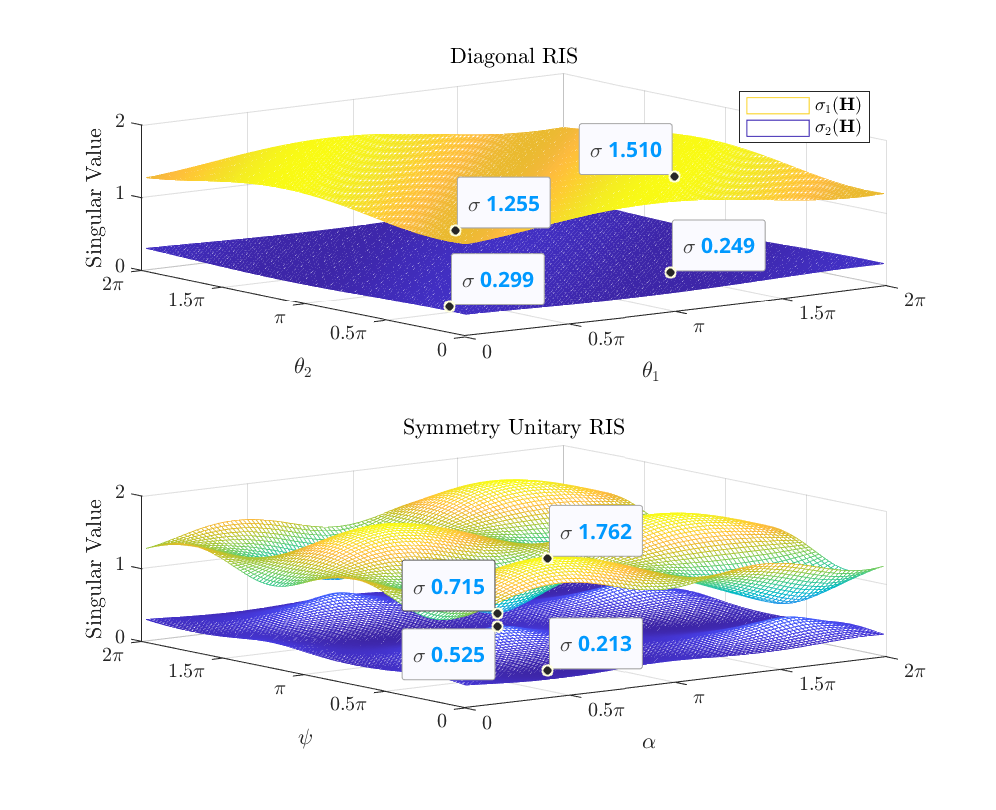
\includegraphics[width=\columnwidth]{assets/simulation/pc_singular_toy.eps}
			\caption{Channel singular value shaping by diagonal and symmetry unitary \gls{ris} for $(N^\mathrm{T}, N^\mathrm{S}, N^\mathrm{R}) = (2, 2, 2)$ without direct link.}
			\label{sm:pc_singular_toy}
		\end{figure}
		Fig.~\ref{sm:pc_singular_toy} illustrates all possible channel singular values achieved by diagonal and symmetry unitary \gls{ris}.
		Despite using the same number of elements and parameters, \gls{bd} \gls{ris} provides much wider dynamic ranges of $\sigma_1(\mathbf{H})$ and $\sigma_2(\mathbf{H})$ than diagonal \gls{ris}.
		Larger gaps are expected when the symmetry constraint can be relaxed.

		We then analyze the channel shaping \emph{capability} of \gls{bd} \gls{ris} under specific setups.
		\begin{subsubsection}{Rank-Deficient Channel}
			In rank-deficient channels, \gls{bd} \gls{ris} $\mathbf{\Theta}^\mathrm{B}$ cannot achieve a higher \gls{dof} than diagonal \gls{ris} $\mathbf{\Theta}^\mathrm{D}$.
			This is because $\mathrm{sv}(\mathbf{\Theta}^\mathrm{B}) = \mathrm{sv}(\mathbf{\Theta}^\mathrm{D}) = \boldsymbol{1}$ and
			\begin{equation}
				\begin{split}
					\mathrm{rank}(\mathbf{H})
					& \le \mathrm{rank}(\mathbf{H}^\mathrm{D}) + \mathrm{rank}(\mathbf{H}^\mathrm{B} \mathbf{\Theta} \mathbf{H}^\mathrm{F}) \\
					& \le \mathrm{rank}(\mathbf{H}^\mathrm{D}) + \min \bigl( \mathrm{rank}(\mathbf{H}^\mathrm{B}), \mathrm{rank}(\mathbf{\Theta}), \mathrm{rank}(\mathbf{H}^\mathrm{F}) \bigr).
				\end{split}
			\end{equation}
			% However, \gls{bd} \gls{ris} can still guarantee a higher rate at finite \gls{snr}.
			Note \gls{bd} \gls{ris} can still provide a higher indirect \gls{snr} as shown in Fig.~\ref{sm:pc_power_sx} and \ref{sm:pc_power_bond}.
		\end{subsubsection}


		\begin{subsubsection}{Rank-1 Indirect Channel}
			The indirect channel is rank-1 iff the forward or backward channel is rank-1.
			Let $\mathbf{H}^\mathrm{F} = \sigma^\mathrm{F} \mathbf{u}^\mathrm{F} {\mathbf{v}^\mathrm{F}}^\mathsf{H}$ without loss of generality.
			In this case, the channel Gram matrix can be written as Hermitian-plus-rank-1:
			\begin{equation}
				\mathbf{G} \triangleq \mathbf{H} \mathbf{H}^\mathsf{H} = \mathbf{Y} + \mathbf{z} \mathbf{z}^\mathsf{H},
			\end{equation}
			where $\mathbf{Y} \triangleq \mathbf{H}^\mathrm{D} (\mathbf{I} - \mathbf{v}^\mathrm{F} {\mathbf{v}^\mathrm{F}}^\mathsf{H}) \mathbf{H}^\mathrm{D} = \mathbf{T} \mathbf{T}^\mathsf{H}$ and $\mathbf{z} \triangleq \sigma^\mathrm{F} \mathbf{H}^\mathrm{B} \mathbf{\Theta} \mathbf{u}^\mathrm{F} + \mathbf{H}^\mathrm{D} \mathbf{v}^\mathrm{F}$.
			Regardless of \gls{ris} size and structure\footnote{A similar conclusion was made for diagonal \gls{ris} in \cite{Semmler2023}.}, its $n$-th ($n \ge 2$) eigenvalues are bounded by the Cauchy interlacing formula \cite{Golub2013}
			\begin{equation}
				\lambda_1(\mathbf{Y}) \ge {\color{blue}\lambda_2(\mathbf{G})} \ge \lambda_2(\mathbf{Y}) \ge \ldots \ge \lambda_{N-1}(\mathbf{Y}) \ge {\color{blue}\lambda_N(\mathbf{G})} \ge \lambda_N(\mathbf{Y}).
			\end{equation}
			The equivalent singular value inequality is
			\begin{equation}
				\sigma_1(\mathbf{T}) \ge {\color{blue}\sigma_2(\mathbf{H})} \ge \sigma_2(\mathbf{T}) \ge \ldots \ge \sigma_{N-1}(\mathbf{T}) \ge {\color{blue}\sigma_N(\mathbf{H})} \ge \sigma_N(\mathbf{T}).
				\label{iq:singular_value_interlacing}
			\end{equation}
			\eqref{iq:singular_value_interlacing} implies that, if the indirect channel is rank-1, then the \gls{ris} can at most enlarge the $n$-th ($n \ge 2$) channel singular value to the $(n-1)$-th singular value of $\mathbf{T}$.
			Note that the largest channel singular value is unbounded with a sufficiently large \gls{ris}.
		\end{subsubsection}

		\begin{subsubsection}{Fully-Connected \glsentryshort{ris} Without Direct Link}
			Denote the singular value decomposition of forward / backward channels as $\mathbf{H}^{\mathrm{B}/\mathrm{F}} = \mathbf{U}^{\mathrm{B}/\mathrm{F}} \mathbf{\Sigma}^{\mathrm{B}/\mathrm{F}} {\mathbf{V}^{\mathrm{B}/\mathrm{F}}}^\mathsf{H}$.
			The composite channel is
			\begin{equation}
				\mathbf{H} = \mathbf{H}^\mathrm{B} \mathbf{\Theta} \mathbf{H}^\mathrm{F} = \mathbf{U}^\mathrm{B} \mathbf{\Sigma}^\mathrm{B} \mathbf{X} \mathbf{\Sigma}^\mathrm{F} {\mathbf{V}^\mathrm{F}}^\mathsf{H},
			\end{equation}
			where $\mathbf{X} = {\mathbf{V}^\mathrm{B}}^\mathsf{H} \mathbf{\Theta} \mathbf{U}^\mathrm{F}$.
			% Since unitary matrices are closed under multiplication,
			\begin{proposition}
				In this case, the singular value bounds on $\mathbf{H}$ are equivalent to the singular value bounds on $\mathbf{BF}$, where $\mathbf{B}$ and $\mathbf{F}$ are arbitrary matrices with singular values $\mathbf{\Sigma}^\mathrm{B}$ and $\mathbf{\Sigma}^\mathrm{F}$.
				% The only singular value bounds applied here are those apply to the singular value bound of $\mathbf{F}\mathbf{B}$
			\end{proposition}
			\begin{proof}
				We first observe that singular value control problem can be solved w.r.t. unitary $\mathbf{X}$ and retrieved by $\mathbf{\Theta} = \mathbf{V}^\mathrm{B} \mathbf{X} {\mathbf{U}^\mathrm{F}}^\mathsf{H}$.
				Also, $\mathrm{sv}(\mathbf{U}^\mathrm{B} \mathbf{\Sigma}^\mathrm{B} \mathbf{X} \mathbf{\Sigma}^\mathrm{F} {\mathbf{V}^\mathrm{F}}^\mathsf{H}) = \mathrm{sv}(\bar{\mathbf{U}}^\mathrm{B} \mathbf{\Sigma}^\mathrm{B} \mathbf{\bar{V}}{{}^\mathrm{B}}^\mathsf{H} \bar{\mathbf{U}}^\mathrm{F} \mathbf{\Sigma}^\mathrm{F} \mathbf{\bar{V}}{{}^\mathrm{F}}^\mathsf{H}) = \mathrm{sv}(\mathbf{BF})$ where $\bar{\mathbf{U}}^{\mathrm{B}/\mathrm{F}}$ and $\bar{\mathbf{V}}^{\mathrm{B}/\mathrm{F}}$ are arbitrary unitary matrices.
			\end{proof}
			The problem now becomes, given $\mathbf{\Sigma}^\mathrm{B}$ and $\mathbf{\Sigma}^\mathrm{F}$, what can we say about the singular value of $\mathbf{BF}$.
			One comprehensive answer is Horn's inequality \cite{Bhatia2001}: for all admissible triples $(I, J, K)$,
			\begin{equation}
				\prod_{k \in {K}} \sigma_k(\mathbf{BF}) \leq \prod_{i \in {I}} \sigma_i(\mathbf{B}) \prod_{j \in {J}} \sigma_j(\mathbf{F}).
			\end{equation}
			It gives upper bound on the largest singular value and lower bound on the smallest singular value:
			\begin{align}
				\sigma_1(\mathbf{BF}) \le \sigma_1(\mathbf{B}) \sigma_1(\mathbf{F}) \label{iq:singular_value_largest}\\
				\sigma_N(\mathbf{BF}) \geq \sigma_N(\mathbf{B}) \sigma_N(\mathbf{F}) \label{iq:singular_value_smallest}.
			\end{align}
			Another useful result is introduced in \cite{Hogben2013}: for all $p>0$,
			\begin{equation}
				\sum_n \sigma_n^p(\mathbf{BF}) \leq \sum_n \sigma_n^p(\mathbf{B}) \sigma_n^p(\mathbf{F}) \label{iq:singular_value_power_sum}.
			\end{equation}
			When $p=2$, it implies the channel energy is upper bounded by the sum of element-wise power product of the forward and backward channels, as illustrated in Fig.~\subref*{sm:pc_power_bond_nd}.
			Interestingly, \eqref{iq:singular_value_largest}--\eqref{iq:singular_value_power_sum} are simultaneously tight when $\mathbf{X} = \mathbf{I}$ and $\mathbf{\Theta} = \mathbf{V}^\mathrm{B} {\mathbf{U}^\mathrm{F}}^\mathsf{H}$.
			This solution was claimed in \cite{Bartoli2023} to achieve channel capacity, but it is not true at moderate \gls{snr}.
			% In \cite{Bartoli2023}, the authors claimed this solution also achieves channel capacity but it is
		\end{subsubsection}





		Finally, we characterize the \emph{Pareto front} of channel singular values via optimization approach.
	\end{subsection}
\end{section}


\bibliographystyle{IEEEtran}
\bibliography{library.bib}
\end{document}
